\documentclass[tikz, convert={outfile=rap.svg}]{standalone}
\usepackage{amsmath}
\usepackage[sfdefault]{FiraSans}
\usepackage{FiraMono}
\usetikzlibrary{arrows, fit, shapes}
\begin{document}
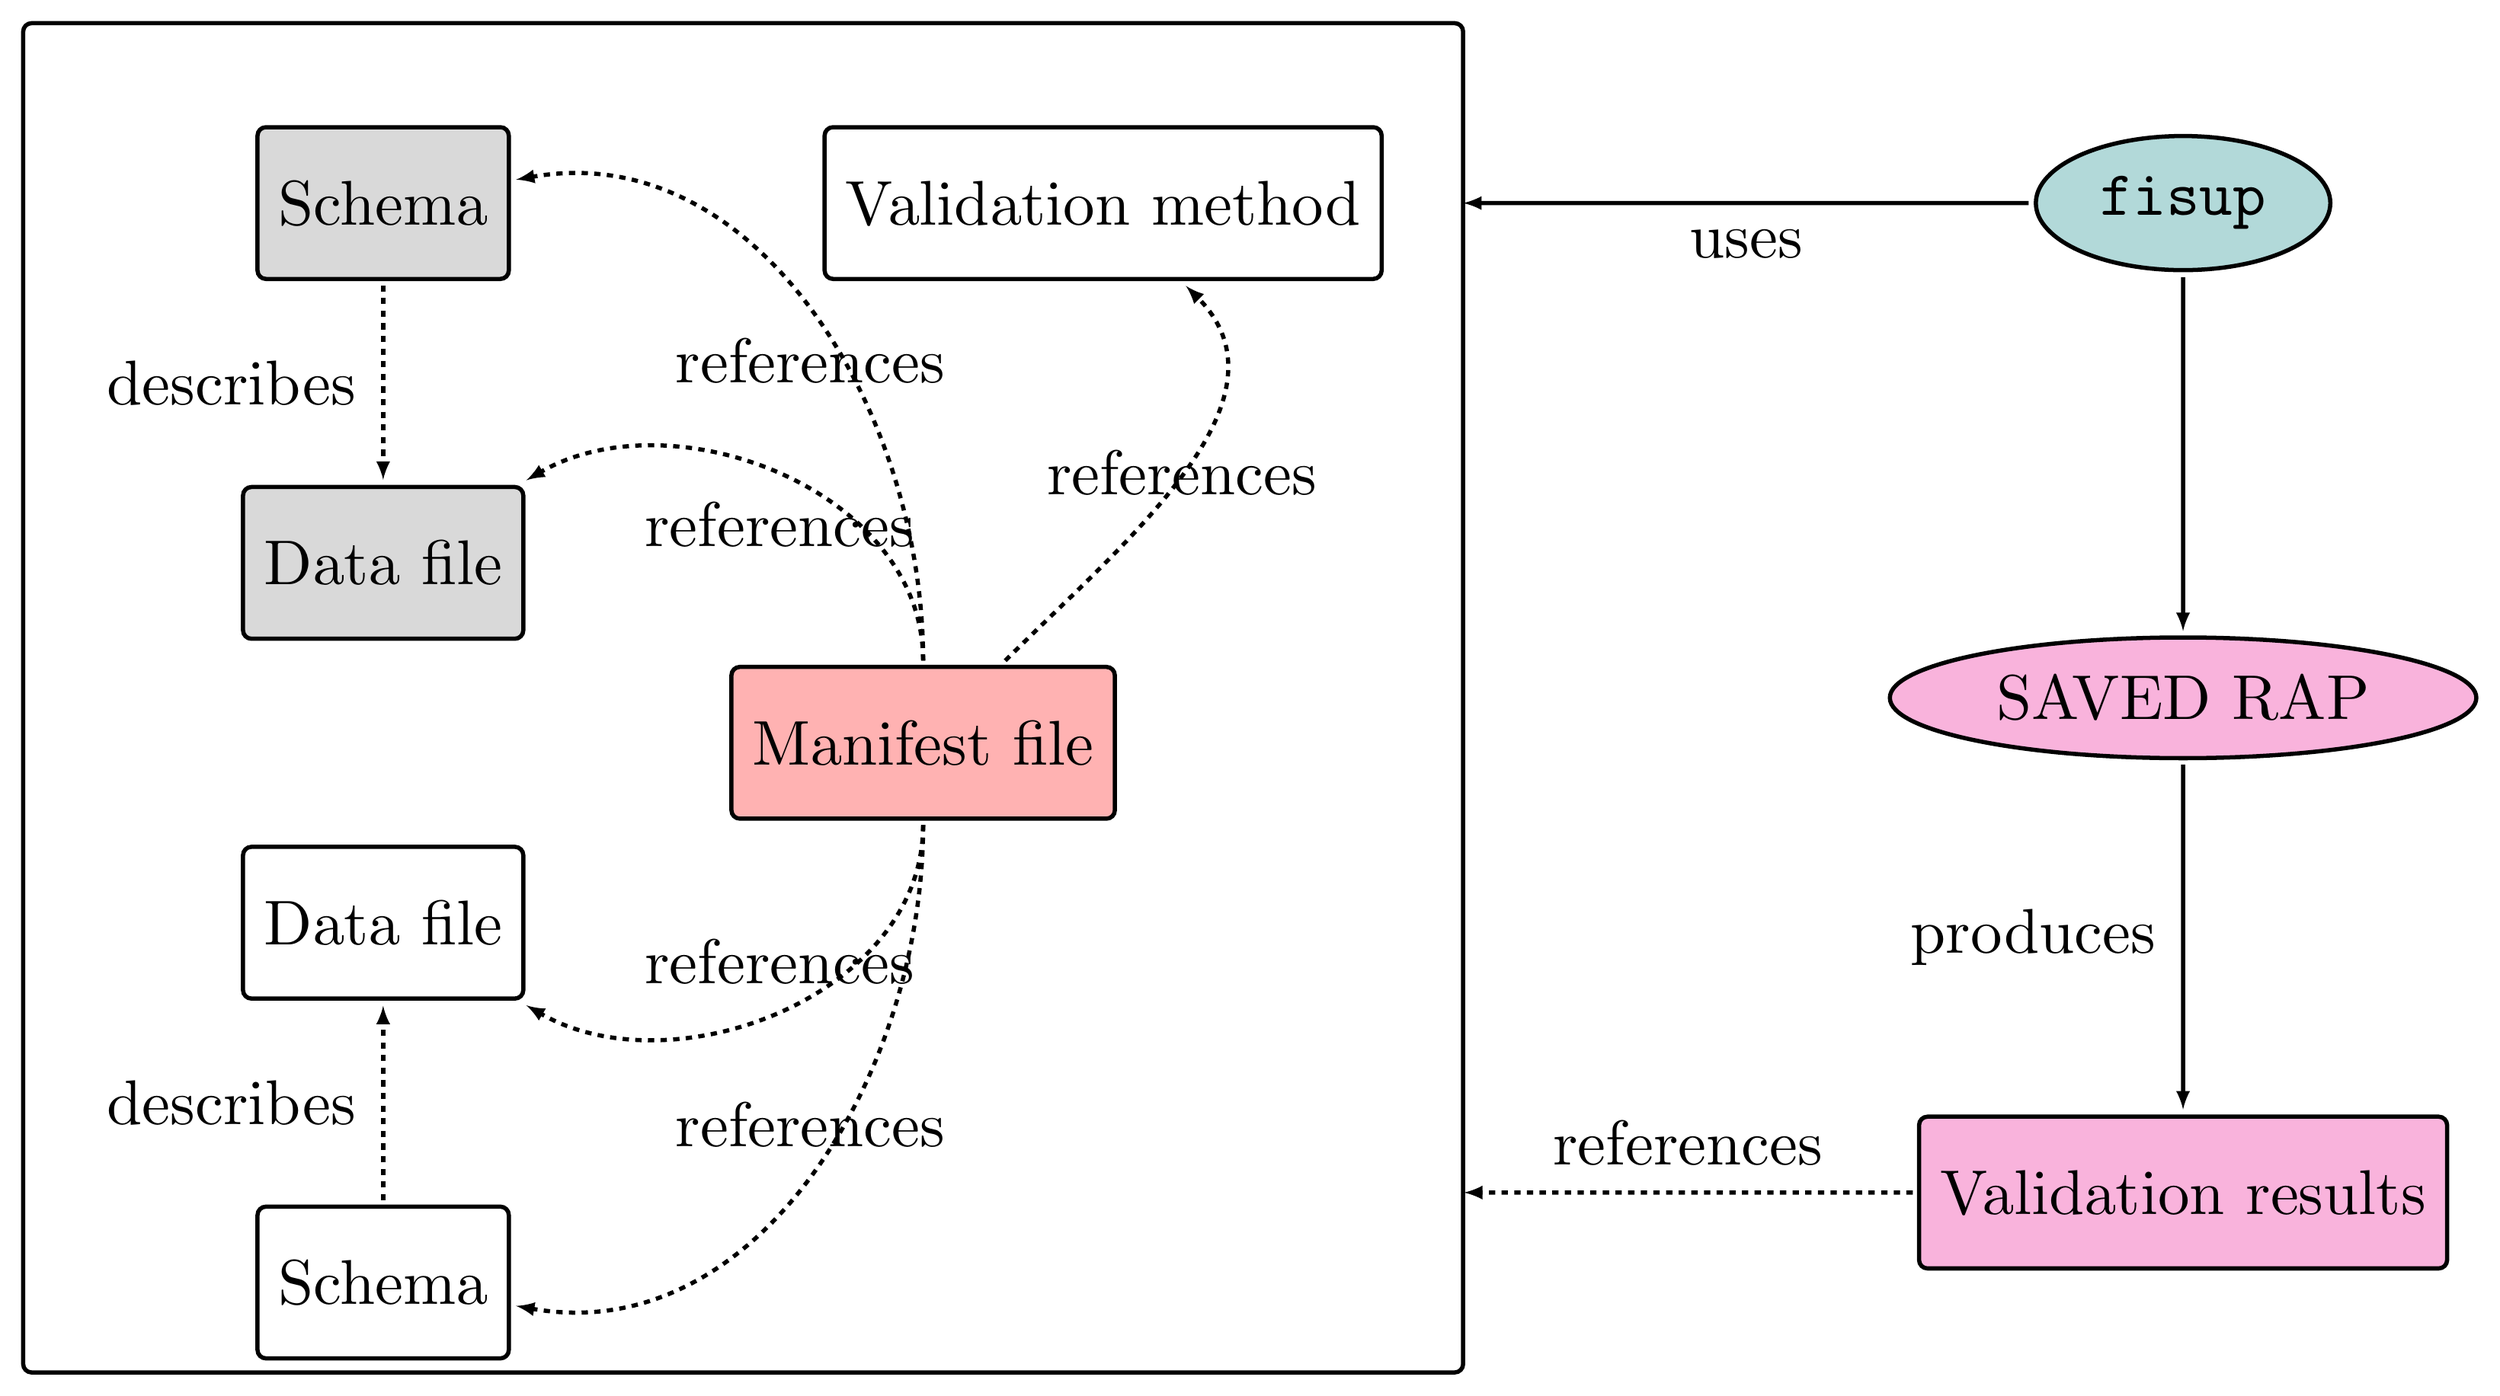
\begin{tikzpicture}[
    line width=0.7mm,
    scale=3,
    box/.style={draw,ellipse},
    data/.style={draw,rounded corners,minimum height=2\baselineskip},
    refd/.style={draw,dashed,-latex,shorten >=0.4pt},
    used/.style={draw,latex-,shorten >=0.4pt},
    proc/.style={draw,-latex,shorten >=0.4pt},
    transform shape]
  \draw[rounded corners] (-2,-3.5) rectangle (6,4);
  \node[data,fill=gray!30] at (0,1) (densout) { Data file };
  \node[data,fill=gray!30] (densschm) at (0,3) { Schema };
  \draw[refd] (densschm) -- node[left] { describes } (densout);
  \node[data] at (0,-1) (obsout) { Data file };
  \node[data] (obsschm) at (0,-3) { Schema };
  \draw[refd] (obsschm) -- node[left] { describes } (obsout);
  \node[data,fill=red!30] (manif) at (3,0) { Manifest file };
  \path[refd] (manif) edge[out=90,in=10] node[below] { references } (densschm);
  \path[refd] (manif) edge[out=90,in=30] node[below] { references } (densout);
  \path[refd] (manif) edge[out=-90,in=-10] node[above] { references } (obsschm);
  \path[refd] (manif) edge[out=-90,in=-30] node[above] { references } (obsout);
  \node[data] (job) at (4,3) { Validation method };
  \path[refd] (manif) edge[out=45,in=315] node { references } (job);
  \node[box,fill=teal!30] (fisup) at (10,3) { \texttt{fisup} };
  \path[used] (6,3) -- node[below] { uses } (fisup);
  \node[box,fill=magenta!30] (rap) at (10,0.25) { SAVED RAP };
  \draw[used] (rap) -- (fisup);
  \node[data,fill=magenta!30] (out) at (10,-2.5) { Validation results };
  \path[proc] (rap) edge node[left] { produces } (out);
  \path[refd] (out) edge node[above] { references } (6,-2.5);
\end{tikzpicture}
\end{document}
